% Target: 35 pages
% Current: 3

\chapter{Adapters in Machine Translation}
\label{chap:adaptmt}
The aim of this Chapter is to understand the impact of pre-trained models when fine-tuning machine translation model with adapters. Specifically, we are interested to understand the contribution of good representation in the pre-training language model to the adapters during the fine-tuning as well as understanding the capability of adapters to perform under pre-trained models that theoretically have inferior representation. We propose to use Transformer architecture with BERT and manually trained language models as the pre-train weights in both encoder and decoder components while using adapters for the fine-tuning. To be more specific, we divide the experiments into fur different areas:
\begin{itemize}
    \item Use BERT weights\footnote{We use publicly available BERT weights from Huggingface hub \url{https://huggingface.co}} as the pre-train weights (\texttt{Pre-trained BERT})
    \item Use Transformer architecture with BERT configuration and pre-train the models with MLM objective on IWSLT and WMT data (\texttt{Pre-trained Transformer})
    \item Use Transformer architecture with BERT configuration and fully random weights as the pre-train weights (\texttt{Pre-trained random})
    \item Use Transformer architecture with BERT weights as the pre-train weights where the weights are shuffled (\texttt{Pre-trained shuffled})
\end{itemize}

\section{Experiments Setup}
\subsection{Language Model}
\label{ssec:langmodel}
\subsubsection{Dataset}
From \cite{devlin2018bert}, we understand that BERT is trained with billions of words from various sources and domains. However, we do not really know to what point can we stop adding sentences to the pre-training data so that we can reduce the hours of training the model. To achieve the goal, we are reducing the scope of the pre-training data by only restricting the pre-training data from machine translation task with two different domain. In this work, we use a combination of WMT and IWSLT to construct the dataset. Specifically, we are constructing three different dataset with different volumes: 500k and 2 millions number of sentences. Other than that, we also use a standalone IWSLT data for pre-training the model.

The construction of the dataset was done with a simple approach by randomly selecting sentences from either dataset and combine them until we meet the pre-requisites number of sentences that we have mentioned on the previous paragraph.

\subsubsection{Model}
To pre-train the model, we follow the work from \cite{devlin2018bert} by using Masked Language Model (MLM) objective to train the model. Complete illustration can be found in Figure \ref{img:mlmobj}. Essentially on every sentences, some words will be deleted and the job of the model is to predict the missing words. One of the benefit of using this objective compared to the auto-regressive objective that used in other model such as GPT model (\cite{brown2020language,ratford2019language,radford2018improving}) is that we can exploit the bidirectional context when training the model rather than only predicting the words from left-to-right.

\begin{figure}[h]
    {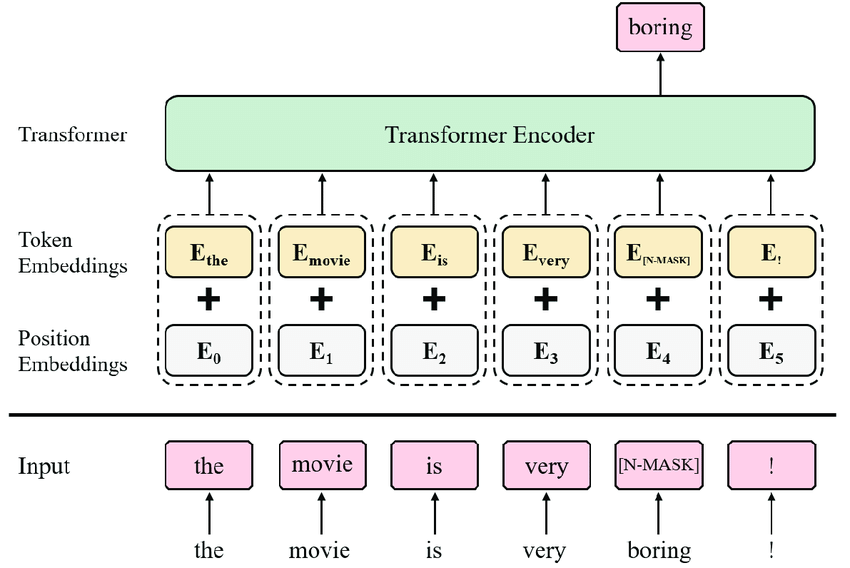
\includegraphics[width=0.95\textwidth]{img/mlm_obj.png}}
    \centering
    \caption{Illustration of MLM objective during the pre-training. Illustration is reprinted from \cite{devlin2018bert}.}
    \label{img:mlmobj}
\end{figure}

We use the default BERT configuration from huggingface to construct the model. A complete list of the hyperparameters can be found on \cref{tab:hyp}.

\begin{table}[]
    \begin{tabular}{@{}lccc@{}}
        \toprule
        \textbf{Name}                   & \textbf{En} & \textbf{De} & \textbf{Description}                                                                         \\ \midrule
        vocab\_size                     & 30522       & 31102       & \begin{tabular}[c]{@{}c@{}}Vocabulary size of the\\ BERT model\end{tabular}                  \\
        hidden\_size                    & 768         & 768         & \begin{tabular}[c]{@{}c@{}}Dimensionality for each\\ of the layers\end{tabular}              \\
        num\_hidden\_layers             & 12          & 12          & \begin{tabular}[c]{@{}c@{}}Number of hidden layers\\ in the transformer\end{tabular}         \\
        num\_attention\_heads           & 12          & 12          & \begin{tabular}[c]{@{}c@{}}Number of attention heads for\\ each attention layer\end{tabular} \\
        intermediate\_size              & 3072        & 3072        & \begin{tabular}[c]{@{}c@{}}Dimensionality of the\\ feed-forward layer\end{tabular}           \\
        hidden\_act                     & gelu        & gelu        & \begin{tabular}[c]{@{}c@{}}The activation function\\ within the layer\end{tabular}           \\
        hidden\_dropout\_prob           &
        0.1                             &
        0.1                             &
        \begin{tabular}[c]{@{}c@{}}The dropout probability\\ for all fully connected layers in\\ the embeddings, encoder,\\ and pooler\end{tabular}                \\
        attention\_probs\_dropout\_prob &
        0.1                             &
        0.1                             &
        \begin{tabular}[c]{@{}c@{}}The dropout ratio for the\\ attention probabilities\end{tabular}                                                                \\ \bottomrule
    \end{tabular}
    \caption{Transformer parameter for English based on \texttt{bert-base-uncased} German based on \texttt{bert-base-german-dbmdz-uncased}}
    \label{tab:hyp}
\end{table}

We train the model until convergence. The definition of convergence in our case for MLM objective is to train the model until the validation loss is no longer improving. Each languages with different number of volumes may end up converging in different steps.

\subsection{Machine Translation}
\subsubsection{Dataset}
In machine translation experiments, there are several scenarios on which we use both WMT and IWSLT dataset. The IWSLT dataset is mainly used for fine-tuning and evaluation of the final model. The WMT, on the other hand, will be combined with IWSLT for training the baseline models. Similar to the language model experiments, we will have three different baselines: IWSLT standalone, IWSLT + WMT (500k), IWSLT + WMT (2 millions). To be more specific, for IWSLT standalone we use the IWSLT dataset for training, evaluation, as well as testing. For the rest of dataset with combination of IWSLT and WMT, we use them for training only while on evaluation and testing we still refer to the IWSLT data alone.

\subsubsection{Model}
We use a sequence-to-sequence architecture described on \cite{vaswani2017attention}. The sequence-to-sequence architecture contains two different components, encoder and decoder. The details and exact figure of this architecture has been described on Chapter 1. The encoder and decoder use the same model and hyperparameters as described in the Section \ref{ssec:langmodel}. The only modification from the original model in language model is in the decoder side. We understand that on the encoder side all the self-attention layer will only refer to the neighbors of theh current layer only for gathering the context. On the other hand, for the decoder, we need further context by including the representation from the eneocder as the extra features. For this reason, an extra layer such as \texttt{cross\_attention} layer is introduced in the decoder and will be trained from scratch for any experiments.

\section{Experiments Results}
This section will discuss the result obtained for machine translation tasks. First, in Section \ref{ssec:adaptcomp}, we conduct the comparative study of using adapters with different scenarios. Second, in Section \ref{ssec:randshuff}, we perform a study by replacing the BERT model with a different BERT version where the weights are shuffled. We continue the study of understanding the adapters behaviour by replacing the pre-trained weights with completely random set of weights and not using the BERT model. Finally, in Section \ref{ssec:randpre}, we perform the experiments to understand the contribution of the total number of sentences used in the pre-training.

\subsection{Adapters Comparison}
\label{ssec:adaptcomp}
\subsubsection{Experiment Setup and Motivation}
We are first trying to understand the contribution of adapters by performing the comparison of models that trained and fine-tuned with different size of datasets. The definition of dataset is the same as have already explained on the previous section. There are three different categories of dataset that is used in two different ways:
\begin{itemize}
    \item Used by baseline model to train the model from scratch
    \item Used for pre-training and later fine-tuned on IWSLT dataset
\end{itemize}

\subsubsection{Experiment Results}
\begin{figure}[h]
    {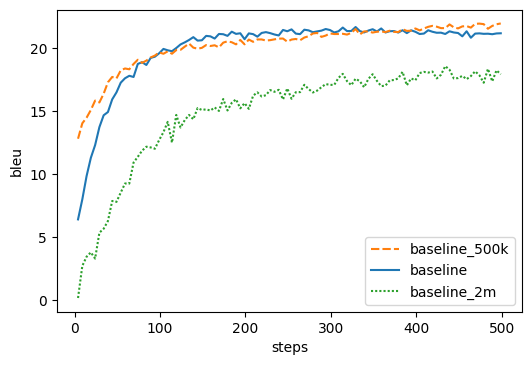
\includegraphics[width=0.95\textwidth]{img/baseline.png}}
    \centering
    \caption{
        Comparison between baseline models trained with different size of datasets. \texttt{baseline} represents the model trained only using IWSLT; \texttt{baseline\_500k} represents the model trained using IWSLT and WMT with total of 500k sentence pairs; \texttt{baseline\_2m} represents the model trained using IWSLT and WMT with total of 2 million sentence pairs.}
    \label{img:basecomp}
\end{figure}

In this section, we compare the result of the baseline models with the models that are fine-tuned with adapters. From Figure \ref{img:basecomp}, adding more data to the baseline models does not necessarily improve the performance. We suspect the models require more time to train to get better performance. There is a clear gap between \texttt{baseline\_2m} and the rest of the baseline models. \texttt{baseline} and \texttt{baseline\_500k} performs really well from the start while \texttt{baseline\_2m} lag behind. We suspect this is the effect of including more sentences from different domains. \texttt{baseline\_500k} is the best mix given the training time constraint. It provides a balance in between not overfitting in the correct domain and not too much data out of the domain. \texttt{baseline\_2m} shows the impact on domain difference. It does not perform well on IWSLT but it is growing and has a chance to improve the performance further. At a later stage, the \texttt{baseline\_2m} output would deserve manual evaluation, because the lower bleu may not necessarily reflect a lower quality, we can see some of the result in Table \ref{tab:qtvout}.

To see the impact of including adapters, we compare the result on different sizes of pre-training used for the base model. The base models are then fine-tuned with the adapters module on the IWSLT data. As we can see from Figure \ref{img:adpcomp}, BERT achieves the best performance from the earlier steps compared to the rest of the pre-training size. In contrast to the baseline models, we see the benefit of adding more sentences to the pre-training. We can see the performance progression between the model that was trained using 500k data has lower performance than the one using 2 million data. On the other hand, models that only use IWSLT as the pre-training data suffers from performance degradation in the middle of the fine-tuning. We observed that this is due to the gradient explosion on the cross-attention layer. The IWSLT model eventually managed to achieve a similar performance to the 500k model in the later steps.
\begin{figure}[h]
    {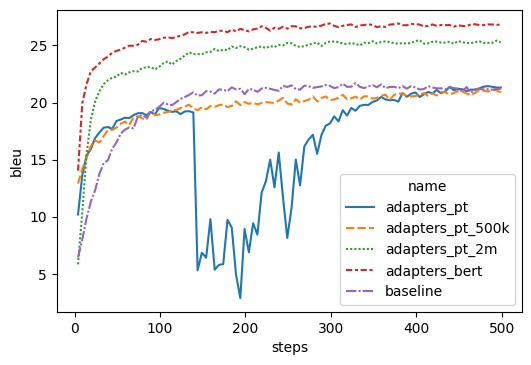
\includegraphics[width=0.95\textwidth]{img/adapterscomparison.png}}
    \centering
    \caption{
        % \XXX{Could you include baseline curve, too? This is rather important for comparison given the lack of the stopping criterion.}
        Comparison between adapters pre-trained with different size of datasets. \texttt{baseline} represents the model trained only using IWSLT; \texttt{adapters\_pt} represents the model pre-trained only using IWSLT; \texttt{adapters\_pt\_500k} represents the model pre-trained using IWSLT and WMT with total of 500k sentence pairs; \texttt{adapters\_pt\_2m} represents the model pre-trained using IWSLT and WMT with total of 2 million sentence pairs; \texttt{adapters\_bert} represents the model that uses BERT weights.}
    \label{img:adpcomp}
\end{figure}

\begin{table*}[]
    \centering
    \begin{tabular}{@{}c@{}}
        \toprule
        \textbf{Random Weights + Adapters}                                                                                                                                                                                                             \\ \midrule
        \begin{tabular}[c]{@{}c@{}}\textbf{input}: wir tanzen im tempel und werden zu gott. \& quot ;\\ \textbf{prediction}: we \& apos ; re going to be able to become god. \& quot ;\end{tabular}                                                    \\ \midrule
        \begin{tabular}[c]{@{}c@{}}\textbf{input}: aber gleichzeitig hatten sie eine klare kenntnis des waldes, \\ die erstaunlich war.\\ \textbf{prediction}: but at the same time, they had a clear of the audience \\ who was amazing.\end{tabular} \\ \midrule
        \begin{tabular}[c]{@{}c@{}}\textbf{input}: es ist so wunderbar. ihr musst es beschutzen. \& quot ;\\ \textbf{prediction}: it \& apos ; s wonderful. you have to protect it. \& quot ;\end{tabular}                                             \\ \bottomrule
    \end{tabular}
    \caption{Prediction results from randomly set pre-trained model fine-tuned with adapters}
    \label{tab:qtrand}
\end{table*}

\subsection{Random and Shuffled Pre-training Weights}
\label{ssec:randshuff}
\subsubsection{Experiment Setup and Motivation}
To show to what extent the Adapter approach benefits from the exact pre-trained weights vs. some of their general distribution properties vs. just the network structure, we conduct experiments where we start by shuffling BERT weights. To perform the experiment, we separate the weights initialization into two approaches: 1) We shuffled the weights from a column perspective. This means in all the weights matrices in the BERT network, we shuffled the weights by preserving columns but shuffling their order. 2) We shuffled the weights from both column and row perspectives.

Furthermore, we also conduct experiments where randomly set weights on all base network layers as the pre-training models. During the fine-tuning, we only update the weights of the adapter and keep the rest of the weights intact.

\subsubsection{Experiment Results}
We can see from Figure \ref{img:shfrndcmp} that the performance of the model that uses random weights as the pre-training model is more stable than the one using shuffled BERT weights. Both of the shuffled BERT models suffer from gradient explosion similar to the IWSLT model we show in the previous section. Although the performance of the random model is still below the baseline model, it is interesting to see that only fine-tuning adapters and the cross-attention layer manage to achieve a reasonable BLEU score, considering that the pre-training models do not contain any meaningful information.
\begin{figure}[h]
    {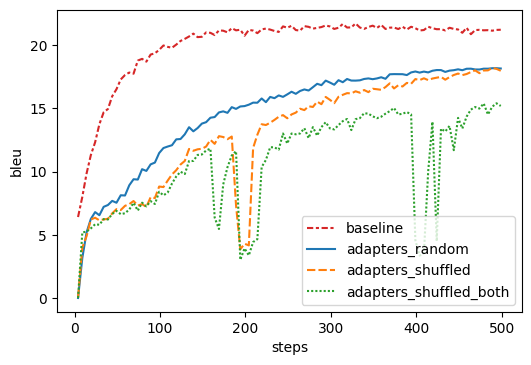
\includegraphics[width=0.95\textwidth]{img/randomshuffled.png}}
    \centering
    \caption{Comparison between adapters using shuffled BERT and random weights as the pre-trained models. \texttt{baseline} represents the model trained only using IWSLT; \texttt{adapters\_random} represents the model pre-trained only using random weights; \texttt{adapters\_shuffled} represents the model pre-trained using column-wise shuffled BERT model; \texttt{adapters\_shuffled\_both} represents the model pre-trained using shuffled BERT model.}
    \label{img:shfrndcmp}
\end{figure}

Since we are relying on the base model with a random set of weights, there is a possibility that our method prone to fallacy that the method only works in a single random seed. To ensure that we perform a robust experiemnt, we repeat the random experiments 10 times with 10 different random seeds. We can see from the result in Figure \ref{img:rndmseed} that all the random seed performs similarly to one and another.

\begin{figure}[h]
    {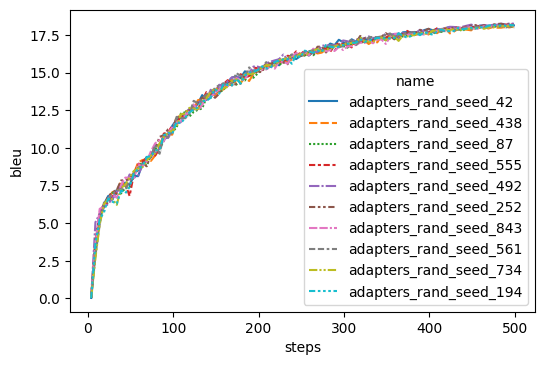
\includegraphics[width=0.95\textwidth]{img/adapter_random_multiseed.png}}
    \centering
    \caption{Comparison of different random seed for randomly set weights based models.}
    \label{img:rndmseed}
\end{figure}

\subsection{Random Pretraining vs. Out-of-Domain Data}
\label{ssec:randpre}
\subsubsection{Experiment Setup and Motivation}
In this experiment, we use the same setup as in the Section \ref{ssec:adaptcomp} and \ref{ssec:randshuff}. Specifically, we are interested to investigate the performance of the random weights model compared to the baseline model. We notice that from the previous experiments, we can gain a reasonable score with the random weights model, in this experiment we are conducting further study the performance relative to the baseline where the models were trained using a mix of WMT and IWSLT. The goal of this comparative study is to understand whether we can gain benefit by only fine-tuning a small number of weights (adapters) vs training the whole transformer model with bigger data size.

\subsubsection{Experiment Results}
We further analyze the random weights by comparing the result with the best performing, baseline, and transformer models we pre-trained ourselves. From Figure \ref{img:rndbslcmp}, we can see that the performance of the random model achieves a similar result to the baseline model that uses 2 million training sentence pairs.
This tells us that training the whole models with bigger data does not necessarily improve the model's performance. It may need further tuning to gain benefits of bigger data and bigger model. We can see the result of using random weights as a potential alternative for training the model with small data such as IWSLT.
While the performance is still far from the baseline that is trained using only IWSLT data, this result shows the base model's structure helps the adapter achieve a meaningful performance with very small weights required for the fine-tuning.

We perform a quick check to the output of the model in Table \ref{tab:qtrand}. We can see from the first two lines that the model has difficulty to capture complex phrases. On the first row, the model missed \textbf{tanzen im tempel} which means \textbf{dancing in the temple}. For the second row, the model confuses \textbf{knowledge of the forest} and output \textbf{audience instead}. Furthermore, the model also does not translate the word \textbf{kenntnis} and makes the translation unclear since the object of the sentence is missing. Despite those mistakes, the model still can capture simple sentences as shown on the third row. Another observation that we noticed in the generated output is the tokenization of \texttt{\&quot\;} and \texttt{\&amp\;}. Instead of being treated as a single token, the tokenizer treats the token as three different subword token. We notice that this is due to the inavailability of the aforementioned token in the pre-trained BERT vocabulary.


\begin{figure}[h]
    {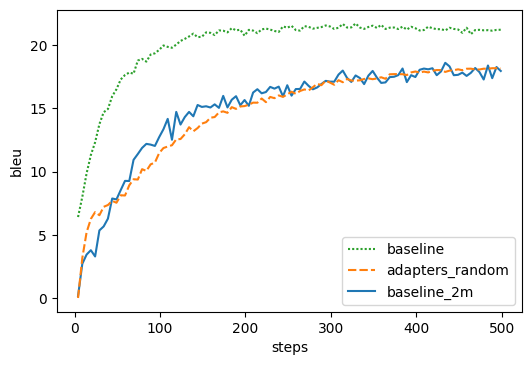
\includegraphics[width=0.95\textwidth]{img/random.png}}
    \centering
    \caption{Comparison between pre-trained random weights and baseline model. \texttt{baseline} represents the model trained only using IWSLT; \texttt{baseline\_2m} represents the baseline model trained with a combination of IWSLT and WMT sentence pairs; \texttt{adapters\_random} represents the model pre-trained only using random weights; \texttt{adapters\_pt\_2m} represents the model pre-trained using IWSLT and WMT with total of 2 million sentence pairs; \texttt{adapters\_bert} represents the model that uses BERT weights}
    \label{img:rndbslcmp}
\end{figure}

\section{Qualitative Comparison}
\begin{sidewaystable*}
    \centering
    \begin{tabular}{|l|l|l|}
        \hline
        \multicolumn{1}{|c|}{\textbf{Baseline IWSLT}}                                                                                                                                                                                                                     &
        \multicolumn{1}{c|}{\textbf{IWSLT + WMT (total 2m)}}                                                                                                                                                                                                              &
        \multicolumn{1}{c|}{\textbf{BERT + Adapters}}                                                                                                                                                                                                                                \\ \hline
        \begin{tabular}[c]{@{}l@{}}\textbf{input}: erinnerst du dich an\\ den patienten\\ mit dem gereizten rachen? \\ \textbf{prediction}: do you remember\\ reading to the patients? on the\end{tabular}                                                                &
        \begin{tabular}[c]{@{}l@{}}\textbf{input}: erinnerst du dich an\\ den patienten\\ mit dem gereizten rachen? \\ \textbf{prediction}: do you remember\\ the patient with the tingling\\ revenge?\end{tabular}                                                       &
        \begin{tabular}[c]{@{}l@{}}\textbf{input}: erinnerst du dich an\\ den patienten\\ mit dem gereizten rachen? \\ \textbf{prediction}: remember the\\ patient with\\ the bruised remorse?\end{tabular}                                                                          \\ \hline
        \begin{tabular}[c]{@{}l@{}}\textbf{input}: großartig, sagte ich.\\ legte auf.\\ \textbf{prediction}: great, i said.\\ got up..\end{tabular}                                                                                                                       &
        \begin{tabular}[c]{@{}l@{}}\textbf{input}: großartig, sagte ich.\\ legte auf.\\ \textbf{prediction}: great, i said.\\ put on..\end{tabular}                                                                                                                       &
        \begin{tabular}[c]{@{}l@{}}\textbf{input}: großartig, sagte ich.\\ legte auf.\\ \textbf{prediction}: great, i said.\\ put it down.\end{tabular}                                                                                                                              \\ \hline
        \begin{tabular}[c]{@{}l@{}}\textbf{input}: - - aber in unserer\\ entdeckung der welt, haben\\ wir alle arten unterschiedlicher\\ methoden.\\ \textbf{prediction}: but in our discovery\\ of the world, we \& apos ;\\ ve got all sorts of different\end{tabular}  &
        \begin{tabular}[c]{@{}l@{}}\textbf{input}: - - aber in unserer\\ entdeckung der welt, haben\\ wir alle arten unterschiedlicher\\ methoden.\\ \textbf{prediction}: - - but in our discovery\\ of the world, we have\\ all kinds of different methods.\end{tabular} &
        \begin{tabular}[c]{@{}l@{}}\textbf{input}: - - aber in unserer\\ entdeckung der welt, haben\\ wir alle arten unterschiedlicher\\ methoden.\\ \textbf{prediction}: but in our discovery\\ of the world, we have\\ all sorts of different ways of doing\\ things.\end{tabular} \\ \hline
    \end{tabular}
    \caption{Prediction results from 1) Baseline model trained with only IWSLT data; 2) Pre-trained model with adapters where we pre-train the model with IWSLT and WMT with a total of 2 million pre-training data; 3) BERT with adapters.}
    \label{tab:qtvout}
\end{sidewaystable*}
We perform a sanity check to compare the generated results on some of our models. This sanity check is to check the errors produced by the models on different techniques.
From Table \ref{tab:qtvout}, we can see for the first example none of the models managed to generate the correct result. However, BERT + adapters and 2 million pre-trained base models manage to generate the proper context where the result is still discussing \textbf{the patient}. The wrong part is when the model generates an incorrect translation regarding the patient's disease. The second example shows that the BERT + adapters create the correct and better output than the other models. The final example shows that BERT + adapters generate an interesting output where it manages to remove unimportant characters such as \texttt{--} and produce readable output. There may be a slightly different opinion on this example as the 2 million pre-trained base model generate a more concise output.
